\section{Resultados}

El sintonizador de parámetros obtuvo los mejores parámetros para las dos instancias analizadas, los cuales se muestran en la Tabla \ref{tab:mejoresparam}.

\begin{table}[!htb]
\begin{center}
\begin{tabular}{|l|r|r|r|r|r|}
\hline
Instancia & \pmejores & \pclones & \preemplazo & \popsize & \clonsize \\
\hline
\hline
Mandl & 1.00 & 0.25 & 0.30 & 150 & 200 \\
\hline
Mumford0 & 0.25 & 0.25 & 0.30 & 150 & 150 \\
\hline
\end{tabular}
\end{center}
\caption{Valores entregados por el sintonizador para cada instancia.}
\label{tab:mejoresparam}
\end{table}

De acuerdo a estos resultados, se puede apreciar que el parámetro \pmejores{} se mantuvo en el valor por defecto para Mandl, pero disminuyó al mínimo posible en Mumford0. Probablemente, esto se debe a que la red de Mumford0 es más grande y se tiene mejor esperanza de mejorar las soluciones si se toma una fracción de las mejores soluciones para pasar al proceso de mutación.

El mejor valor para el parámetro \pclones{} fue asignado al mínimo posible en ambas instancias, lo que indica que se toma una fracción pequeña de valores para almacenar en el conjunto de memoria, lo que tiene una ventaja computacional al evitar almacenar soluciones que podrían ser eliminadas posteriormente. 

El parámetro \preemplazo{} se mantuvo en el valor por defecto sugerido en ambas instancias y probablemente es el mejor valor para un \textit{trade-off} entre exploración y explotación en una vecindad de soluciones candidatas.

Los tamaños de población, reflejados en los parámetros \popsize{} y \clonsize{} aumentaron con respecto a los valores por defecto. Al comparar las cantidades de ambas poblaciones, se cumple que el tamaño de la población de clones siempre es mayor o igual al tamaño de la población de cada generación.


Al realizar experimentos para la instancia de Mandl con los mejores valores de los parámetros con 15 semillas distintas, se pueden apreciar los frentes de Pareto resultantes de 4 de ellas en las Figuras \ref{fig:paretoMandl1} y \ref{fig:paretoMandl2}. Además, información adicional de apoyo referente a estos frentes se encuentra en la Tabla \ref{tab:dataFrenteMandl}. 

\begin{figure}[p]
\centering
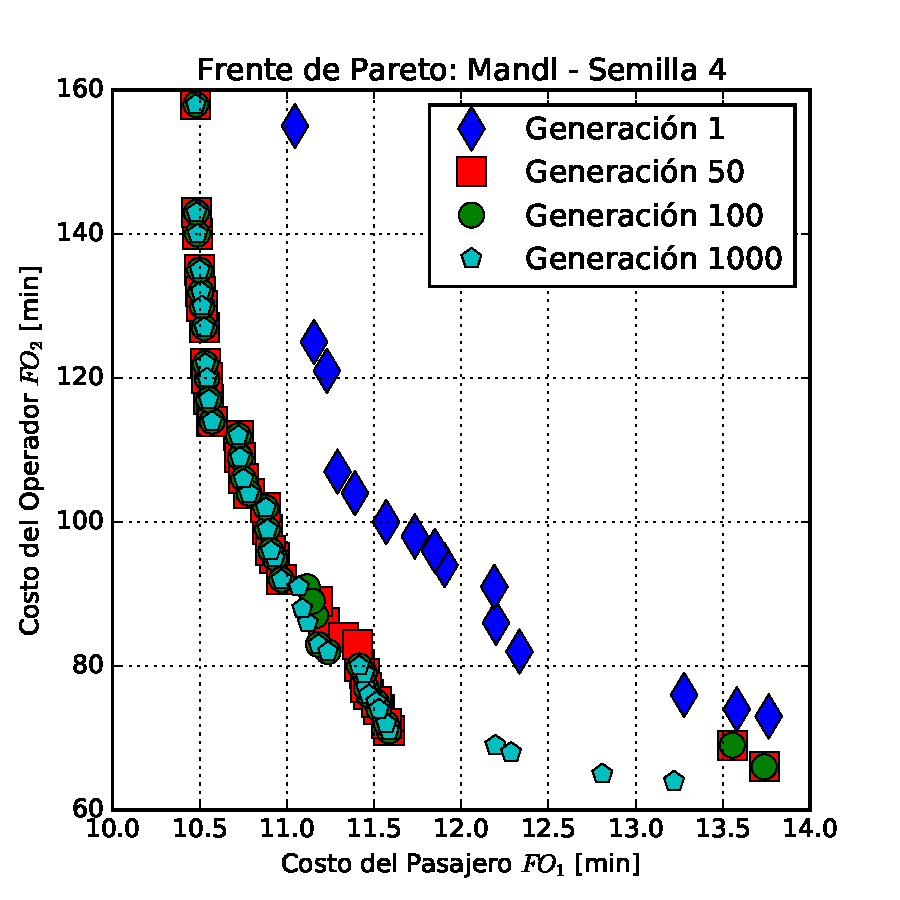
\includegraphics[width=0.79\textwidth]{img/frente_Mandl_s4}
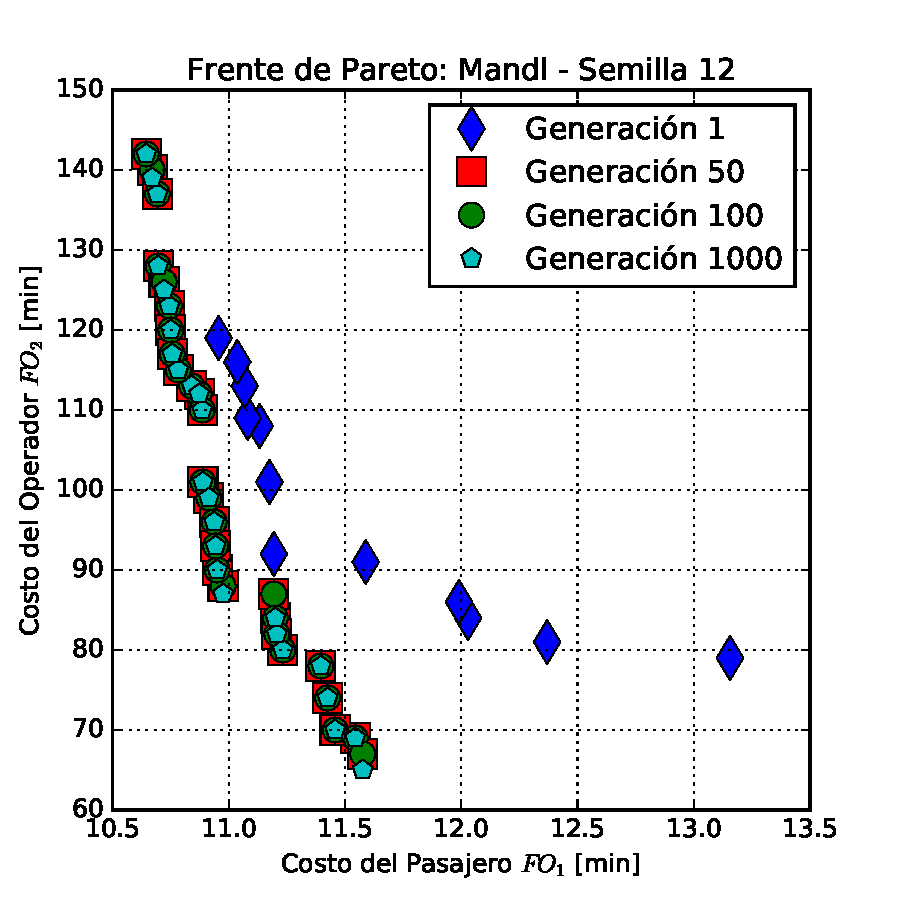
\includegraphics[width=0.79\textwidth]{img/frente_Mandl_s12}
\caption{Frente de Pareto para Mandl con semillas 4 y 12.}
\label{fig:paretoMandl1}
\end{figure}

\begin{figure}[p]
\centering
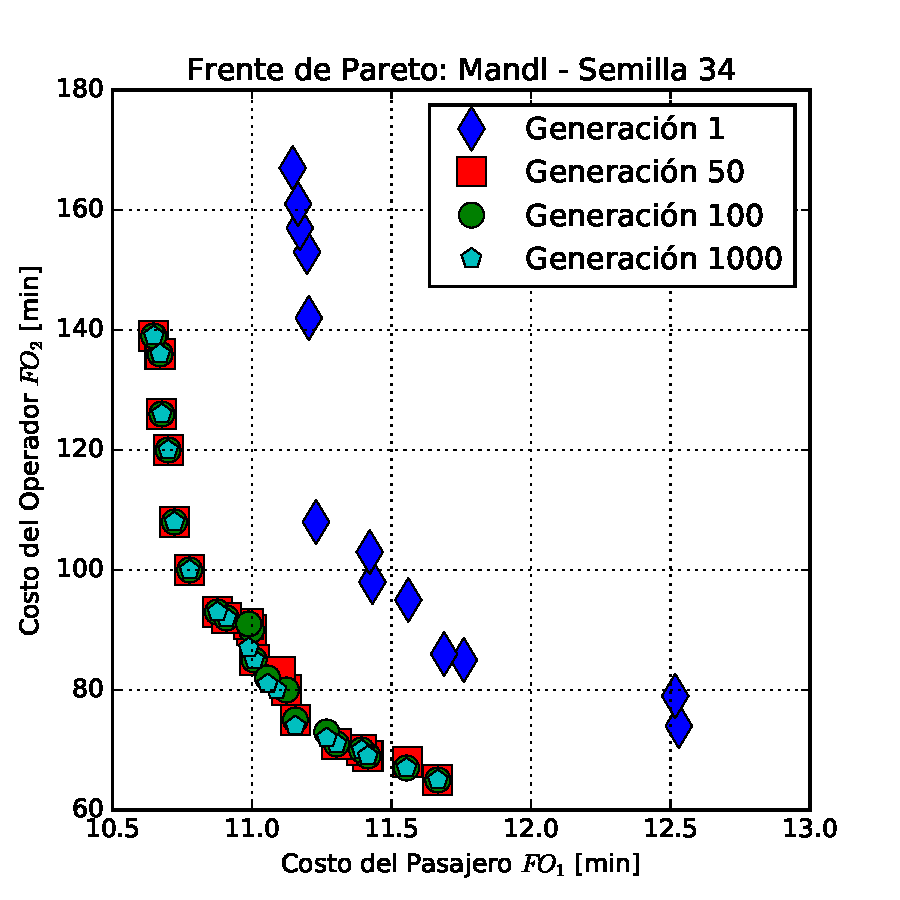
\includegraphics[width=0.79\textwidth]{img/frente_Mandl_s34}
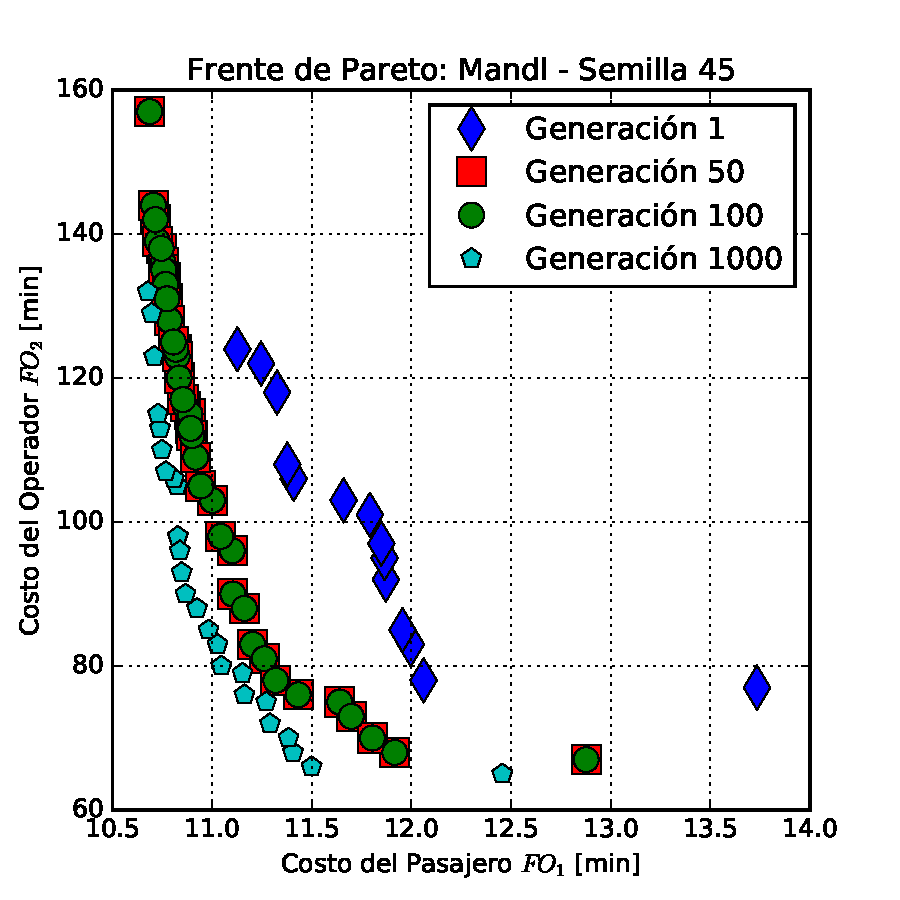
\includegraphics[width=0.79\textwidth]{img/frente_Mandl_s45}
\caption{Frente de Pareto para Mandl con semillas 34 y 45.}
\label{fig:paretoMandl2}
\end{figure}

En general, en todos los casos se puede ver visualmente que los frentes de Pareto se acercan a los mínimos de ambas funciones. El cambio en los frentes de Pareto, se ve reflejado en un aumento en el hipervolumen a medida que avanzan las generaciones. Además, aparecen nuevas soluciones que son mínimos para una u otra función objetivo. La cantidad de soluciones de los frentes aumenta a medida que transcurren generaciones en el algoritmo inmune. Luego, se puede afirmar que el alogoritmo inmune es capaz de explorar lugares distintos en búsqueda de soluciones distintas a las que se generan inicialmente y además, se logran mejorar las soluciones existentes. Más específicamente, por medio de la información de la Tabla \ref{tab:dataFrenteMandl} se destaca para este algoritmo en específico la aparición de muchas soluciones idénticas en los frentes de pareto. 

Se puede observar, a modo general que desde la generación 50 y la generación 100 la soluciones totales son el doble de las soluciones únicas. En la generación 1000, las soluciones únicas representa entre un 10\% y un 30\% de las soluciones totales. En esta instancia se mantiene la tendencia de que la semilla que genera más soluciones únicas es la que tiene más soluciones totales. No existe una correlación entre un mayor hipervolumen con más soluciones únicas/totales en el frente. 

Finalmente, el tiempo para una instancia fue medido desde el inicio del algoritmo hasta la finalización de una generación. Tiempos menores en etapas prematuras del algoritmo suelen derivar en un tiempo total de cómputo menor para el algoritmo completo. Notar que al término de la generación 1 han transcurrido cerca de 20 segundos desde el inicio del algoritmo, donde este tiempo está destinado a la generación del conjunto inicial de soluciones factibles para iniciar el algoritmo.

\begin{table}[!htb]
\centering
\begin{tabular}{|r|r|r|r|r|r|}
\hline
Semilla & Generación & Sol. Únicas & Sol. Totales & Hipervolumen & Tiempo [s]\\ 
\hline \hline
4 & 1 & \textbf{15} & \textbf{15} & 702.207 & 26 \\ \hline
45 & 1 & 14 & 14 & 692.819 & 25 \\ \hline
12 & 1 & 12 & 12 & \textbf{714.867} & \textbf{22} \\ \hline
34 & 1 & 13 & 13 & 704.389 & \textbf{22} \\ \hline \hline
4 & 50 & 34 & 34 & 833.746 & 334 \\ \hline
45 & 50 & \textbf{36} & \textbf{36} & 809.110 & 344 \\ \hline
12 & 50 & 27 & 27 & 821.737 & 347 \\ \hline
34 & 50 & 19 & 19 & \textbf{836.426} & \textbf{325} \\ \hline\hline
4 & 100 & 35 & 65 & 834.683 & 645 \\ \hline
45 & 100 & \textbf{36} & \textbf{70} & 809.110 & 663 \\ \hline
12 & 100 & 27 & 27 & 821.737 & 683 \\ \hline
34 & 100 & 20 & 37 & \textbf{836.769} & \textbf{634} \\ \hline \hline
4 & 1000 & \textbf{37} & \textbf{335} & 847.025 & 6770 \\ \hline
45 & 1000 & 25 & 83 & 833.812 & 6533 \\ \hline
12 & 1000 & 26 & 153 & 830.848 & 6675 \\ \hline
34 & 1000 & 19 & 180 & \textbf{837.087} & \textbf{6357} \\ \hline
\end{tabular}
\caption{Cantidad de soluciones únicas/totales, hipervolumen y tiempo de cómputo en el frente de Pareto para 4 semillas de la instancia Mandl.}
\label{tab:dataFrenteMandl}
\end{table}

En el caso de la instancia Mumford0, se realizó el mismo procedimiento, utilizando 15 semillas distintas con 1000 generaciones y los mejores valores  para los parámetros. Las Figuras \ref{fig:paretoMumford1} y \ref{fig:paretoMumford2} muestra la evolución del frente de Pareto en 4 semillas distintas y la Tabla \ref{tab:dataFrenteMumford0} muestra información adicional respecto a estos frentes.

\begin{table}[!htb]
\centering
\begin{tabular}{|r|r|r|r|r|r|}
\hline
Semilla & Generación & Sol. Únicas & Sol. Totales & Hipervolumen & Tiempo [s]\\  
\hline \hline
4 & 1 & \textbf{15} & \textbf{15} & 7118.92 & \textbf{46} \\ \hline
45 & 1 & 12 & 12 & 7054.21 & 52 \\ \hline
12 & 1 & 9 & 9 & 7125.38 & 55 \\ \hline
34 & 1 & 12 & 12 & \textbf{7392.27} & 49 \\ \hline\hline
4 & 50 & 23 & 23 & 8650.36 & \textbf{1219} \\ \hline
45 & 50 & 20 & 20 & 7502.79 & 1742 \\ \hline
12 & 50 & \textbf{30} & \textbf{30} & \textbf{9185.21} & 1349 \\ \hline
34 & 50 & 22 & 22 & 8874.78 & 1276 \\ \hline\hline
4 & 100 & 26 & 33 & 8740.11 & \textbf{2280} \\ \hline
45 & 100 & 38 & 38 & \textbf{9506.56} & 3062 \\ \hline
12 & 100 & 27 & 30 & 9204.48 & 2622 \\ \hline
34 & 100 & \textbf{42} & \textbf{42} & 9285.58 & 3158 \\ \hline\hline
4 & 1000 & 42 & \textbf{103} & 9064.71 & \textbf{24308} \\ \hline
45 & 1000 & 38 & 38 & 9566.61 & 31216 \\ \hline
12 & 1000 & 64 & 85 & \textbf{9792.15} & 27600 \\ \hline
34 & 1000 & \textbf{65} & 83 & 9691.16 & 27324 \\ \hline\hline
\end{tabular}
\caption{Cantidad de soluciones únicas/totales, hipervolumen y tiempo de cómputo en el frente de Pareto para 4 semillas de la instancia Mumford0.}
\label{tab:dataFrenteMumford0}
\end{table}

\begin{figure}[p]
\centering
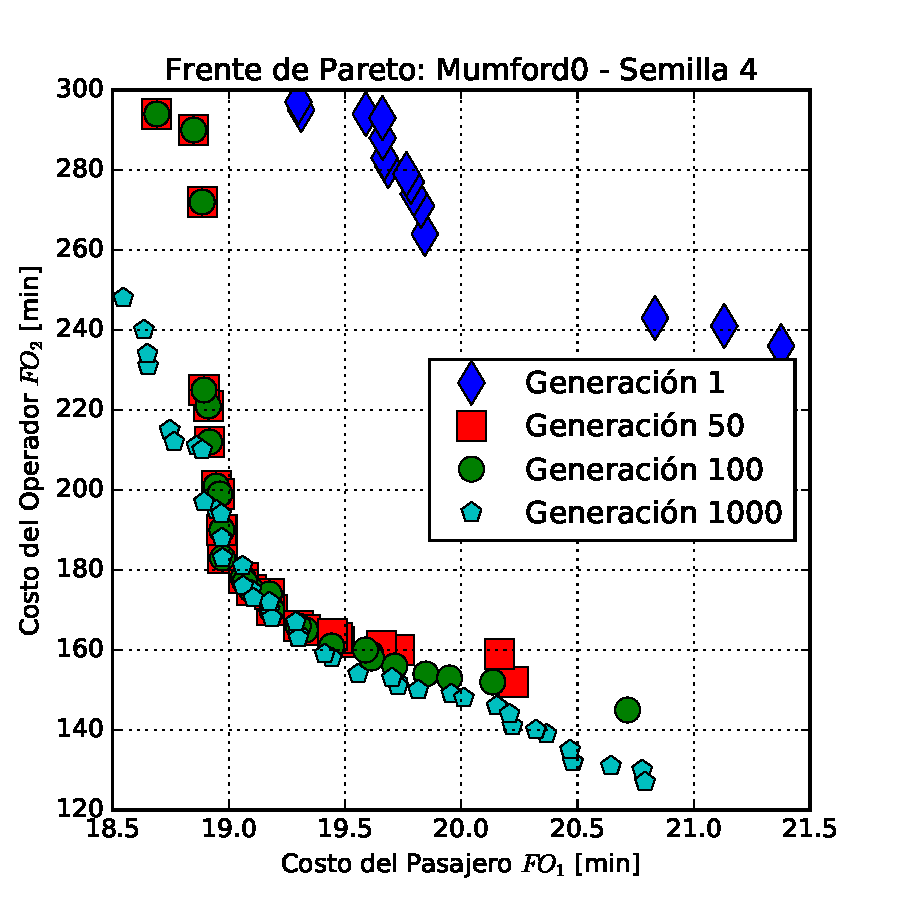
\includegraphics[width=0.79\textwidth]{img/frente_Mumford0_s4}
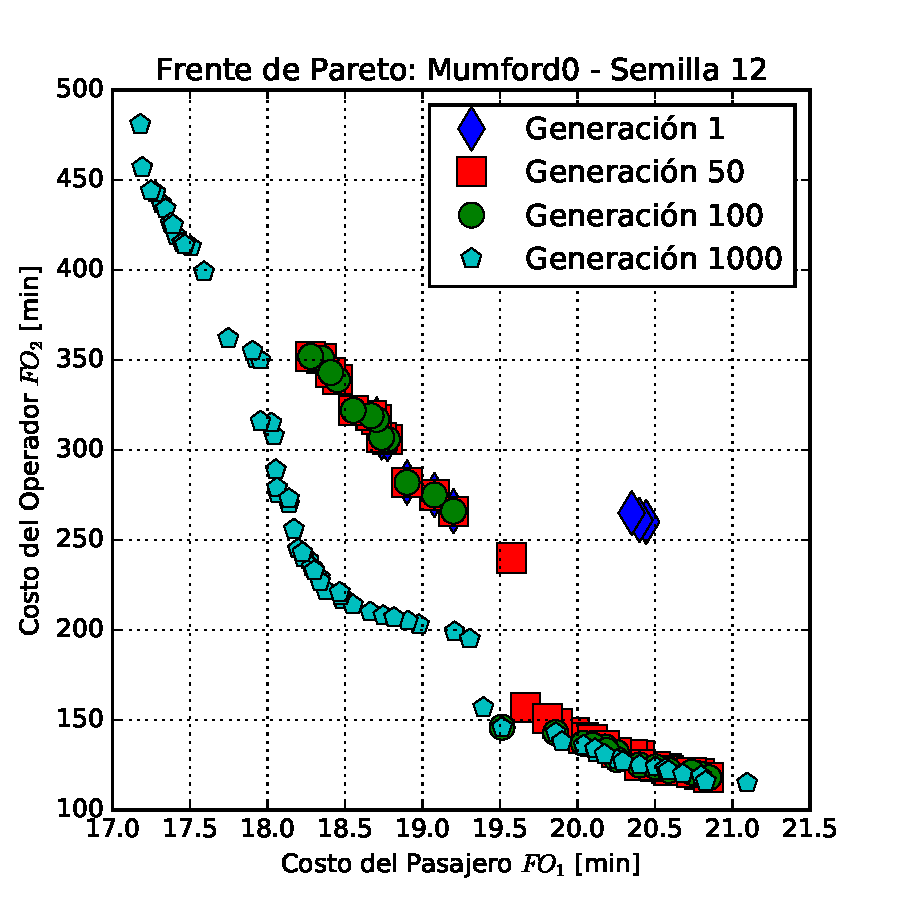
\includegraphics[width=0.79\textwidth]{img/frente_Mumford0_s12}
\caption{Frente de Pareto para Mumford0 con semillas 4 y 12.}
\label{fig:paretoMumford1}
\end{figure}

\begin{figure}[p]
\centering
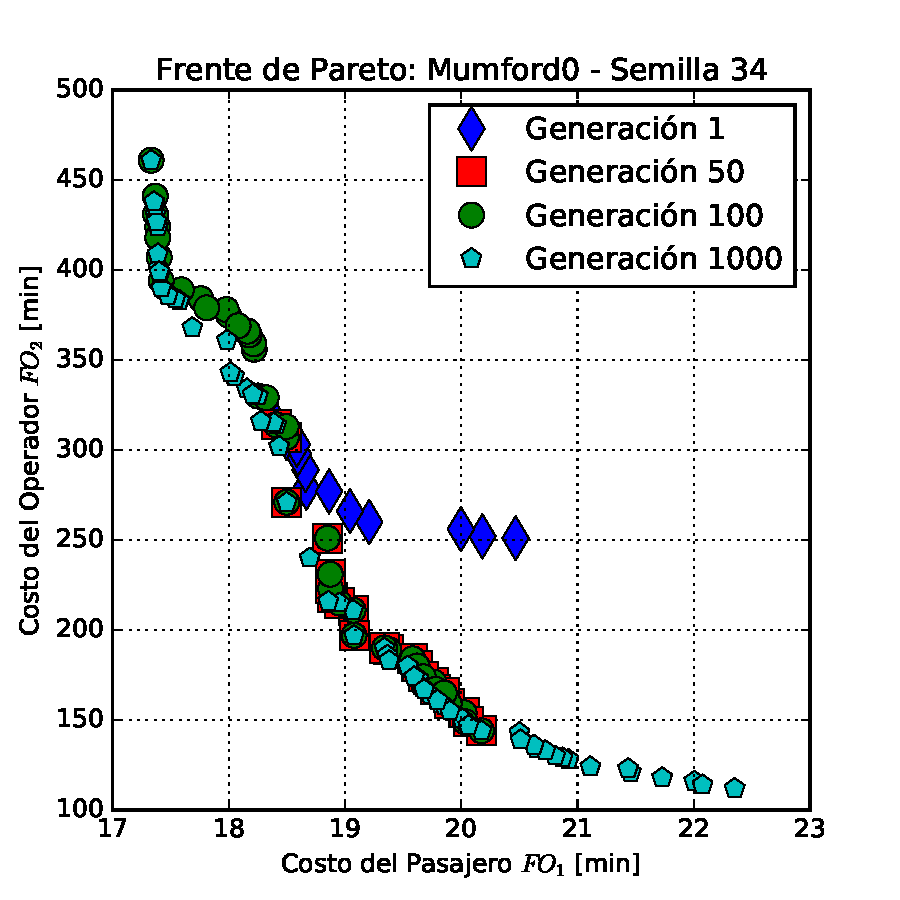
\includegraphics[width=0.79\textwidth]{img/frente_Mumford0_s34}
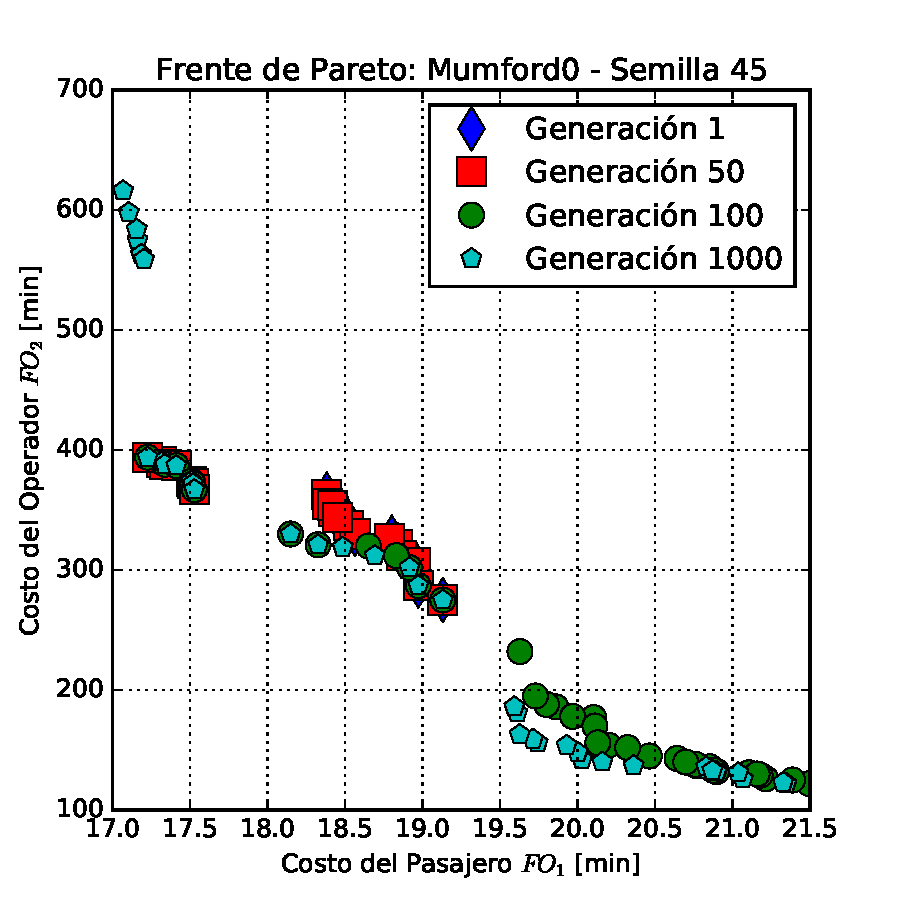
\includegraphics[width=0.79\textwidth]{img/frente_Mumford0_s45}
\caption{Frente de Pareto para Mumford0 con semillas 34 y 45.}
\label{fig:paretoMumford2}
\end{figure}

Se puede apreciar que la evolución de los frentes en las 4 semillas mostradas presenta un comportamiento favorable, ya que se acerca a la región de mínimos en ambas funciones objetivo. Un caso notable a mencionar ocurre con la semilla 4, donde se observa un gran avance a partir del frente inicial en la primera generación hasta el frente obtenido en la generación 50.



\begin{table}[!htb]
\begin{center}
\begin{tabular}{|p{0.14\textwidth}|p{0.36\textwidth}|p{0.50\textwidth}|}
\hline
\multirow{2}{*}{Instancia} & \multicolumn{2}{c|}{Mejor solución para pasajeros (sintonización)} \\
\cline{2-3}
 & Costos & Rutas\\
\hline
\hline
Mandl & $C_p = 10.4778$\newline $C_o = 158$ \newline (semilla=4) & 9-15-6-3-2-1 \newline 3-2-5-4-6-8-10 \newline 4-2-3-6-15-7 \newline 11-10-8-6-3-2-1 \newline 9-15-7-10-11-12-4-2 \newline 11-13-14-10-7 \\
\hline
Mumford0 & $C_p = 17.0681$ \newline $C_o = 616$ \newline (semilla=45) & 8-29-17-3-16-22-7-14-1-13-9-20-18-12 \newline 24-15-2-5-4-10 \newline 27-1-26-12-15-8-3-7-6-16-11 \newline 2-5-25-8-3-30-28-16-22-11-7-6 \newline 18-1-14-7-6-22-3-16-30-28-8-5-2 \newline 27-9-13-20-23-18-1-19-14-7-3-28-17-8 \newline 7-3-11-17-16-28-8-21-15-10 \newline 7-14-19-1-26-23-18-12-4-2-5 \newline 21-8-26-1-13-9 \newline 4-2-5-8-3-7-14-19-13-23-1-20-18-12-15 \newline 30-3-22-6-16-7-14-1-20-18-29-17-28-11-8 \newline 28-11-22-6-7-17-16-3-8-25-2-4-5-15\\
\hline
\end{tabular}
\end{center}
\caption{Mejores soluciones para pasajeros por instancia.}
\label{tab:mejoresfo1}
\end{table}

\begin{table}[!htb]
\begin{center}
\begin{tabular}{|p{0.14\textwidth}|p{0.36\textwidth}|p{0.50\textwidth}|}
\hline
\multirow{2}{*}{Instancia} & \multicolumn{2}{c|}{Mejor solución para operadores (sintonización)}\\
\cline{2-3}
 & Costos & Rutas \\
\hline
\hline
Mandl & $C_p = 13.0501$\newline $C_o = 63$ \newline (semilla=567)  & 11-13-14 \newline 9-15-7 \newline 15-8-6-3-2-4-5 \newline 2-1 \newline 7-10 \newline 12-11-10 \\
\hline
Mumford0 & $C_p = 22.3516$ \newline $C_o = 112$ \newline (semilla=34) & 15-21 \newline 5-25-15 \newline 3-30-11-7 \newline 22-11 \newline 28-17-7-6 \newline 29-26-12 \newline 19-1 \newline 16-7-14 \newline 2-4-10-24 \newline 2-5-8-29-18-19-13-20-9-27 \newline 1-23 \newline 14-1 \\
\hline
\end{tabular}
\end{center}
\caption{Mejores soluciones para operadores por instancia.}
\label{tab:mejoresfo2}
\end{table}


\begin{table}[!htb]
\begin{center}
\begin{tabular}{|p{0.14\textwidth}|p{0.36\textwidth}|p{0.50\textwidth}|}
\hline
\multirow{2}{*}{Instancia} & \multicolumn{2}{c|}{Mejor solución para pasajeros (comparación)} \\
\cline{2-3}
 & Costos & Rutas\\
\hline
\hline
Mandl & $C_p = 10.5164$\newline $C_o = 149$ \newline (semilla=3) &  5-4-6-8-10-7-15-9 \newline  7-15-6-3-2-1 \newline  1-2 \newline  12-11-10-8-6-3-2-1 \newline  14-13-11-10-7 \newline  11-12-4-2-1\\
\hline
Mumford0 & $C_p = 17.3447$ \newline $C_o = 439$ \newline (semilla=2) &  28-30-11-17-29-8-26-12-15-25 \newline  4-2-25-5-8-11-22 \newline  19-18-1-29-8-17-7-11 \newline  8-25-4-12-18-19-14-7-6-16-3 \newline  5-25-2-10-15-24-21-8-3-7 \newline  13-23-19-18-20-9-27-1-26-8-5 \newline  8-21-24-25-5-4-15-2 \newline  26-23-20-1-14-19-18-13-9 \newline  24-21-5 \newline  11-7-14-1-13-9-20-18-12-4-2 \newline  3-22-7-16-11-8-28-17-29-1-13-9 \newline  3-17-29-1-13-9
\\
\hline
\end{tabular}
\end{center}
\caption{Mejores soluciones para pasajeros por instancia.}
\label{tab:mejoresfo1comp}
\end{table}


\begin{table}[!htb]
\begin{center}
\begin{tabular}{|p{0.14\textwidth}|p{0.36\textwidth}|p{0.50\textwidth}|}
\hline
\multirow{2}{*}{Instancia} & \multicolumn{2}{c|}{Mejor solución para operadores (comparación)} \\
\cline{2-3}
 & Costos & Rutas\\
\hline
\hline
Mandl & $C_p = 12.973$\newline $C_o = 63$ \newline (semilla=5678) & 6-3-2-1 \newline  2-4-5 \newline  12-11-10 \newline  11-13-14 \newline  9-15-7-10 \newline  15-8-6 \\
\hline
Mumford0 & $C_p = 21.4104$ \newline $C_o = 116$ \newline (semilla=1234) & 21-15 \newline  14-7-6 \newline  20-13-18-23-1-29 \newline  30-28-17 \newline  5-2-4-10 \newline  19-1 \newline  10-24-15-25 \newline  30-11-7 \newline  21-8-3 \newline  30-3 \newline  15-12-26-23-18-1-27-9 \newline  16-11-22 \\
\hline
\end{tabular}
\end{center}
\caption{Mejores soluciones para operadores por instancia.}
\label{tab:mejoresfo2comp}
\end{table}

